% !TeX document-id = {acd94374-0a5a-4c39-a15c-8f2e56f0151a}
\documentclass[12pt,a4paper, listof=entryprefix, bibliography=totocnumbered,toc=listofnumbered,lof=listofnumbered]{scrartcl}

% WICHTIG!!!
% Pseudokommentar um pdflatex zu erlauben andere Programme zu nutzen z.B. gnuplot
% !TeX TXS-program:compile = txs:///pdflatex/[--shell-escape] 

\usepackage[ngerman]{babel}
\usepackage[utf8]{inputenc}
\usepackage{amsmath}
\usepackage{nccmath}
\usepackage{amsfonts}
\usepackage{amssymb}
\usepackage{graphicx}
\usepackage{fancyhdr}
\usepackage{tabularx}
\usepackage{geometry}
\usepackage{setspace}
\usepackage[right]{eurosym}
\usepackage[printonlyused]{acronym}
\usepackage{subfig}
\usepackage{floatflt}
\usepackage[usenames,dvipsnames]{color}
\usepackage{colortbl}
\usepackage{xcolor}
\usepackage{paralist}
\usepackage{array}
\usepackage{titlesec}
\usepackage{parskip}
\usepackage{picinpar}
\usepackage[pdfpagelabels=true]{hyperref}
\usepackage{listings}
\usepackage{csquotes}
\usepackage{url}
\usepackage{float}
\usepackage{pgfplots}
\usepackage{paralist}
\usepackage[nonumberlist, nogroupskip]{glossaries}

%-----------------------------------------------------------------------------------
% Bibilothek
%-----------------------------------------------------------------------------------
% Einbinden des BibLateX paketes mit Ausgabeeinstellungen
\usepackage[
style=alphabetic,          % Zitierstil
maxbibnames=50,            % alle Autorennamen anzeigen
maxcitenames=4,            % maximale Namen, die im Kürzel angezeigt werden
autocite=inline,           % regelt Aussehen für \autocite (inline=\parancite)
block=space,               % kleiner horizontaler Platz zwischen den Feldern
backref=true,              % Seiten anzeigen, auf denen die Referenz vorkommt
backrefstyle=three+,       % fasst Seiten zusammen, z.B. S. 2f, 6ff, 7-10
date=short,                % Datumsformat
backend = biber,           % Backnend für Aufbereitung
]{biblatex}

%Zusätzliche für Umbrüche für Kleinbuchstaben z.B. in URLs
\appto\UrlBreaks{\do\a\do\b\do\c\do\d\do\e\do\f\do\g\do\h\do\i\do\j
	\do\k\do\l\do\m\do\n\do\o\do\p\do\q\do\r\do\s\do\t\do\u\do\v\do\w
	\do\x\do\y\do\z}


\newcounter{verzeichnis}
\setcounter{verzeichnis}{1}

%Abstände der Einträge
\setlength{\bibitemsep}{1em}     % Abstand zwischen den Literaturangaben
\setlength{\bibhang}{2em}        % Einzug nach jeweils erster Zeile

% Kürzel soll vier Buchstaben der Autoren enthalten statt drei
\DeclareLabelalphaTemplate{
	\labelelement{
		\field[final]{shorthand}
		\field{label}
		\field[strwidth=4,strside=left,ifnames=1]{labelname}
		\field[strwidth=2,strside=left,ifnames=2]{labelname}
		\field[strwidth=1,strside=left]{labelname}
	}
	\labelelement{
		\field[strwidth=2,strside=right]{year}
	}
}

% Bibliothek der Quellen
\bibliography{bib}
\label{bib}

% --------------------------------------------------------------------------------
% Einstellung für Listings
% --------------------------------------------------------------------------------
\lstset{basicstyle=\footnotesize, captionpos=b, breaklines=true, showstringspaces=false, tabsize=2, frame=lines, numbers=left, numberstyle=\tiny, xleftmargin=2em, framexleftmargin=2em}
\makeatletter
\def\l@lstlisting#1#2{\@dottedtocline{1}{0em}{1em}{\hspace{1,5em} Lst. #1}{#2}}
\makeatother

% --------------------------------------------------------------------------------
% Seitenformate
% --------------------------------------------------------------------------------
%Seitenformat
\geometry{a4paper, top=27mm, left=30mm, right=20mm, bottom=32mm, headsep=12mm, footskip=12mm}

% --------------------------------------------------------------------------------
% Metainformationen
% --------------------------------------------------------------------------------
\hypersetup{unicode=false, pdftoolbar=true, pdfmenubar=true, pdffitwindow=false, pdfstartview={FitH},
	pdftitle={Vorlage},
	pdfauthor={Stefan Jung},
	pdfsubject={Abschlussarbeit},
	pdfcreator={\LaTeX\ with package \flqq hyperref\frqq},
	pdfproducer={pdfTeX \the\pdftexversion.\pdftexrevision},
	pdfkeywords={Vorlage},
	pdfnewwindow=true,
	colorlinks=true,linkcolor=black,citecolor=black,filecolor=magenta,urlcolor=black}
\pdfinfo{/CreationDate (D:20141024101000)}
%\pgfplotsset{compat=1.11}

%-----------------------------------------------------------------------------------
% Abkürzungen AKRONYME HIER ERGÄNZEN
%-----------------------------------------------------------------------------------
\glssetwidest{HPPLAN}% Längste Abkürzung für eine korrekte Einrückung

\makenoidxglossaries %Leeres Verzeichnis erstellen

%Abkürzungen hinzufügen
\newacronym{LIP}{LIP}{Labor für Informationstechnik und Produktionslogistik}
\newacronym{OTH}{OTHR}{Ostbayerische Technische Hochschule Regensburg}
\newacronym{CLSP}{CLSP}{Capacitated Lot-Sizing Problem}
\newacronym{HPPLAN}{HPPLAN}{Hauptproduktionsprogrammplanung}
\newacronym{XML}{XML}{Extensible Markup Language}
\newacronym{CSV}{CSV}{Comma-separated values}
\newacronym{GUI}{GUI}{Graphical User Interface}
\newacronym{ANTLR}{ANTLR}{ANother Tool for Language Recognition}

\begin{document}
% --------------------------------------------------------------------------------
% Globale Formateinstellungen
% --------------------------------------------------------------------------------
\onehalfspacing
% Abstände Überschrift
\titlespacing{\section}{0pt}{42pt}{6pt}
\titlespacing{\subsection}{0pt}{12pt}{6pt}
\titlespacing{\subsubsection}{0pt}{12pt}{6pt}

% Kopf- und Fusszeile
\pagestyle{fancy}
\lhead{}\chead{}
\rhead{\thesection\space\contentsname}
\lhead{}\cfoot{}
\rfoot{\ \linebreak \thepage}
\renewcommand{\headrulewidth}{0.4pt}
\renewcommand{\footrulewidth}{0.4pt}

% Nummereriung
\renewcommand{\thesection}{\Roman{section}}
\renewcommand{\theHsection}{\Roman{section}}
\pagenumbering{Roman}

% eigene Farbdefinitionen
\definecolor{lip}{HTML}{3366FF}
\definecolor{grey}{HTML}{ABABAB}

% ---------------------------------------------------------------------------
% Titelseite
% ---------------------------------------------------------------------------
\thispagestyle{empty}

%LIP Schriftzug in eigener Farbe 
\textsf{\begin{minipage}{.69\textwidth}
	\large
	\textcolor{lip}{\textbf{Labor für Informationstechnik und\\Produktionslogistik (LIP)}} %Farbe setzten
	\small 
	\textbf{\\Verfahren, Strategien, Prozesse und IT-Systeme}
	\\Professor Dr.-Ing. Frank Herrmann
\end{minipage}
%Einbinden des OTH Logos mir rechtsbündiger Ausrichtung
\begin{minipage}{.29\textwidth}
	\begin{flushright}
		
\includegraphics[scale=.15]{images/othlogo}\\
	\end{flushright}
\end{minipage}}
 
% Zeilenabstand
\onehalfspacing	

%Beschriftung der Titelseite
\begin{center}

	\vspace*{4cm} %4 cm Vorspann
	\Large
	\textbf{Entwicklerhandbuch für die Themen}\\ %Titel der Arbeit
	\large
	\textbf{Capacitated Lot-Sizing Problem}\\
	\textbf{und}\\
	\textbf{Hauptproduktionsprogrammplanung}\\
		
	\vspace*{7cm} %8 cm Vorspann
	\normalsize
	\begin{center}
	Februar 2015\\
	\textbf{Arnold Christiane \\ Butz Thomas \\ Denzin Timo \\ Eichinger Tobias \\ Gais Dominik \\ Liebich Johannes \\ Schertler Sascha \\ Sonnleitner Daniel \\ Wagner Pilar} %Name des Autors
	
	\end{center}
\end{center}
\pagebreak

% ------------------------------------------------------------------------------
% Inhaltsverzeichnis
% ------------------------------------------------------------------------------
% Inhaltsverzeichnis
\singlespacing %Zeilenabsatnd reduzieren
\setcounter{section}{0}
\setcounter{page}{1}
\addcontentsline{toc}{section}{Inhaltsverzeichnis}%hinzufügen des Inhaltsverzeichnises selbst

\tableofcontents %Ausgabe des Inhaltsverzeichnisses
\pagebreak

% ------------------------------------------------------------------------------
% Setzen der Nummerierungen für Normaltext
% ------------------------------------------------------------------------------
\onehalfspacing %Zeilenabstand auf 1.5
\renewcommand{\thesection}{\arabic{section}} %Arabische Beschriftung für Absatznummern
\pagenumbering{arabic}  %Seitennummerrierung auf arabisch setzen
\setcounter{page}{1}	%Seitenzahl für Inhalt auf 1 setzten
\setcounter{section}{0}
% Kopfzeile mit aktuellem Hauptkapitel darstellen
\renewcommand{\sectionmark}[1]{\markright{#1}} %Section ausgeben
\renewcommand{\subsectionmark}[1]{}            %Subsection nicht ausgeben
\renewcommand{\subsubsectionmark}[1]{}         %Subsubsection nicht ausgeben
\rhead{\rightmark}                             %Ausgabe Rechtsbündig

%------------------------------------------------------------------------------
%	Einführung
%------------------------------------------------------------------------------
\section{Einführung}
Das vorliegende Dokument ist ein Handbuch für Entwickler des \textit{"\gls{HPPLAN}"}-Tools zur Produktionsprogrammplanung im Rahmen der operativen Planung und des Tools \textit{"\gls{CLSP}"} zur dynamischen Losgrößenplanung.


Die Software ist in Java 8 geschrieben und die Benutzeroberfläche wurde mittels JavaFX 8 realisiert.

Nachfolgende Bilder zeigen die Oberflächen der Programme.

\begin{figure}[H]
	\centering
	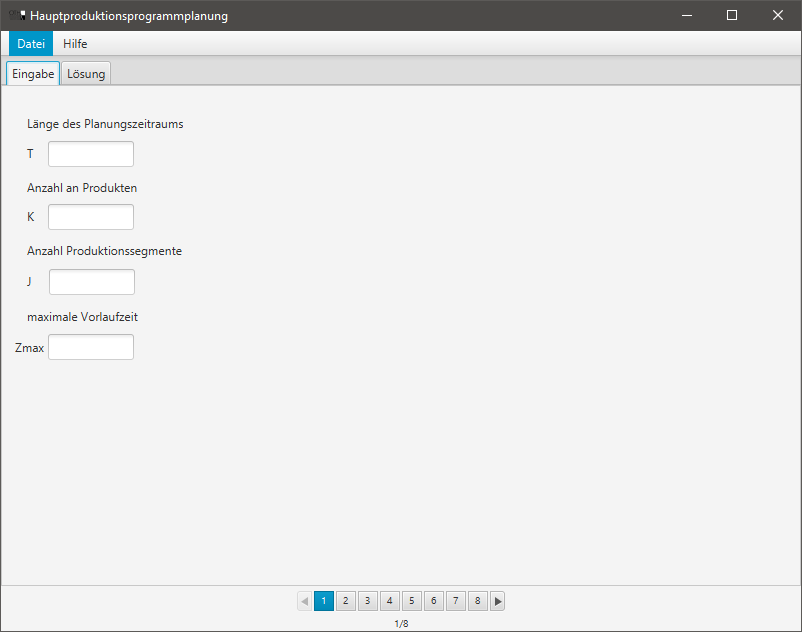
\includegraphics[width=1.0\linewidth]{images/HPPLAN_GUI.png} 
	\captionof{figure}[]{Oberfläche des HPPLAN-Tools}
	\label{fig:hpplangui}
\end{figure}

\begin{figure}[H]
	\centering
	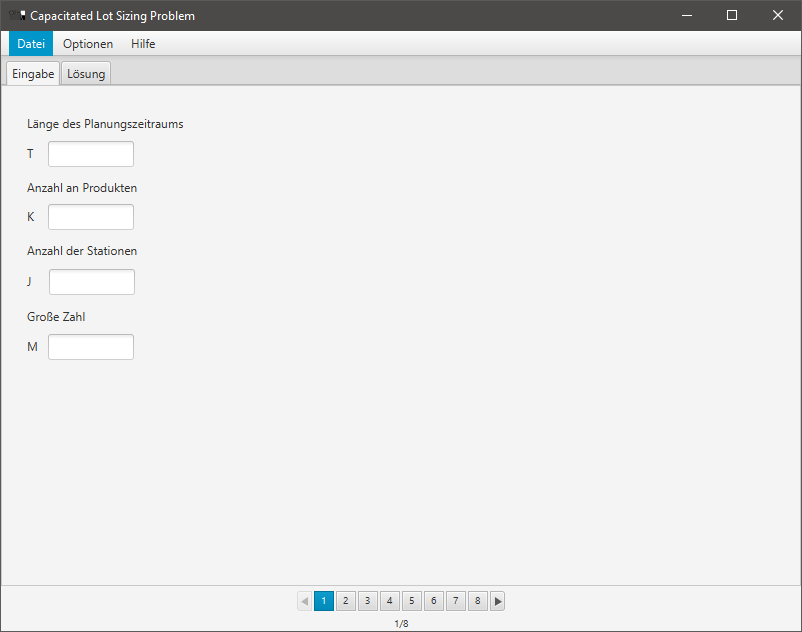
\includegraphics[width=1.0\linewidth]{images/CLSP_GUI.png} 
	\captionof{figure}[]{Oberfläche des CLSP-Tools}
	\label{fig:clspgui}
\end{figure}

\subsection{Aufbau des Dokuments}
Zu Beginn sollen die Problemstellungen der beiden Themen erklärt und die Abläufe der hier verwendeten Verfahren erläutert werden.
\\
Anschließend folgt eine kurze Beschreibung der Funktionen der Software.
\\
Unter dem Punkt Aufbau der Software sollen die einzelnen Komponenten erläutert werden.
\\
Im letzten Kapitel wird auf die Implementierung der einzelnen Komponenten eingegangen.

\subsection{Problemstellung HPPLAN}
Das vorliegende HPPLAN-Tool dient zur Lösung der Hauptproduktionsprogrammplanung. Dabei soll berechnet werden, welche Mengen der einzelnen Produkte in welcher Periode und in welchem Produktionssegment produziert werden sollen. Die Berechnet erfolgt mit dem ILOG-Framework.

\subsection{Problemstellung CLSP}
CLSP ist ein Modell der dynamischen Losgrößenplanung. Es geht dabei von mehreren Produkten aus für die eine begrenzte Produktionskapazität vorhanden ist. Zu ermitteln ist in welcher Periode welche Lose aufgelegt werden sollen und wie groß diese sein sollen. Die Bedarfe der einzelnen Perioden werden dabei als bekannt angenommen. Die CLSP-Berechnung erfolgt ebenfalls mit dem ILOG-Framework.

\subsection{Beschreibung der Software}
Nach dem Start des Tools müssen die Daten zur Berechnung eingegeben werden. Dies geschieht entweder manuell oder durch das Laden einer mit den notwendigen Informationen gefüllten DAT-Datei. Die manuelle Eingabe der Daten ist auf mehrere Seiten aufgeteilt, um die Übersicht zu erhöhen.
\\
Die übergebenen Daten werden in einem temporären Modell gespeichert, an das ILOG-Framework übergeben und in diesem berechnet. Die Ausgabe des Frameworks wird entgegengenommen und in dem Tab "Lösung" ausgegeben.
\\
Detailliertere Information über die Funktionen der beiden Tools finden Sie in den Benutzerhandbüchern.


%------------------------------------------------------------------------------
%	Aufbau der Software
%------------------------------------------------------------------------------

\section{Aufbau der Software}
Im Folgenden werden die verwendete Technik und die Komponenten der Programme vorgestellt. Die Komponenten werden durch Packages realisiert, daher werden in dieser Dokumentation auch die Packagenamen verwendet. Im weiteren Verlauf werden die Begriffe Komponente und Package gleichbedeutend benutzt.

\subsection{Verwendete Techniken}
\paragraph{JavaFX 8}
Die Benutzeroberfläche der Software wurde in JavaFX 8 entwickelt. JavaFX verwendet das Model-View-Controller Prinzip.
\\
Unter dem Java 7 SDK ist die notwendige Bibliothek "jfxrt.jar" noch nicht im Classpath enthalten. Deshalb muss diese zuvor eingebunden werden.

\begin{enumerate}
	\item Einstellungen des Projekts in Eclipse öffnen
	\item Im Reiter Libraries "'Add External JARs"' wählen
	\item Unter [Pfad zum JDK]\textbackslash jdk1.7.[0\textunderscore 06 oder höher]  \textbackslash jre\textbackslash lib findet man die jfxrt.jar
\end{enumerate}
Weitere Informationen unter http://blog.essential-bytes.de/javafx\textunderscore in\textunderscore eclipse/

Um die Gestaltung des \gls{GUI} zu vereinfachen, wird der SceneBuilder verwendet. Der SceneBuilder ist ein Tool zur einfachen Erstellung von JavaFX Layouts. Dabei muss kein Code geschrieben werden, da dies vom SceneBuilder übernommen wird. Das folgende Bild zeigt den SceneBuilder.

\begin{figure}[H]
	\centering
	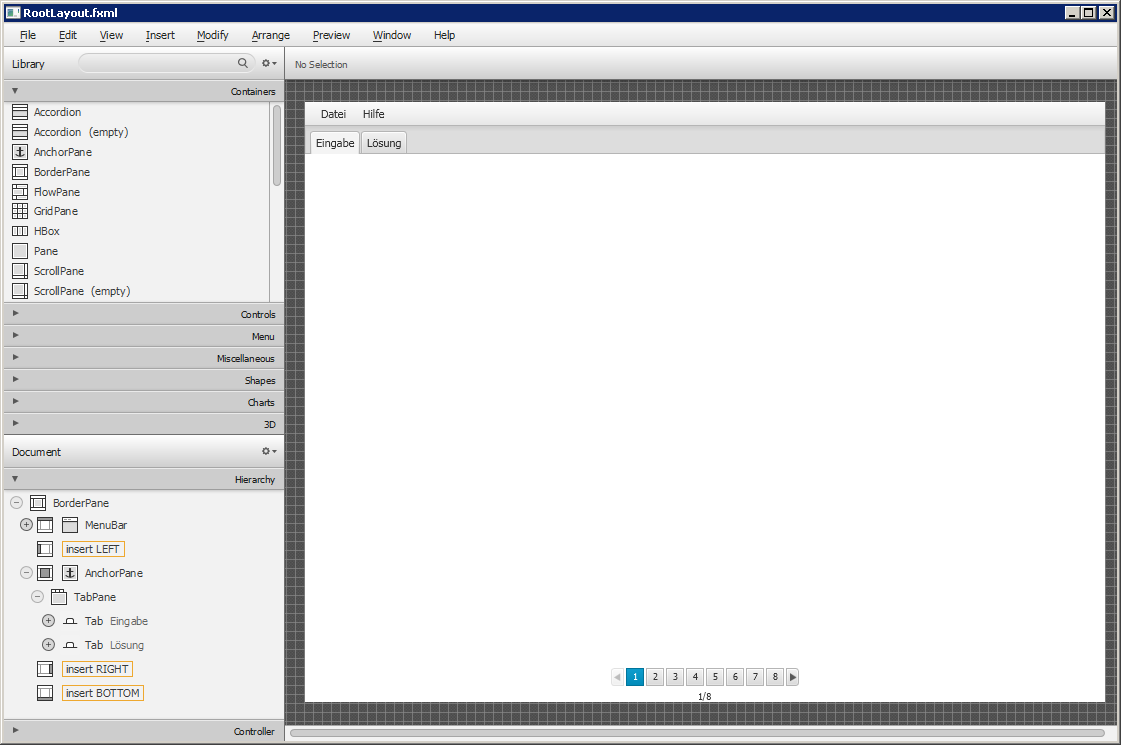
\includegraphics[width=1.0\linewidth]{images/scenebuilder.png} 
	\captionof{figure}[]{Der SceneBuilder}
	\label{fig:scenebuilder}
\end{figure}

Beim Model-View-Controller Prinzip enthält die View lediglich den grafischen Aufbau der Oberfläche. Dieser Aufbau wird einer speziellen \gls{XML} Datei gespeichert, einer sogenannten FXML Datei. 
\\
Eine zugehörige Controller Klasse implementiert die, zur View gehörige, Logik in einer Java Klasse. 
\\
Im Model werden die verwendeten Daten abgespeichert und verwaltet. 
\\
Weder Model noch View enthalten Logik. Dies führt zu einer sauberen Schichtentrennung zwischen Benutzeroberfläche (View), Logik (Controller) und Datenhaltung (Model).
\\
\\
In der FXML-Datei wird die Controller Klasse gesetzt, dadurch kann der Compiler, beim Übersetzten des Programms, Controller und View einander zuordnen. 
Im Folgenden ist zu sehen, wie dies im SceneBuilder umgesetzt werden kann.

\begin{figure}[H]
	\centering
	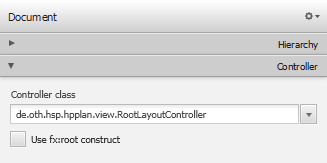
\includegraphics[]{images/controllerClass.png} 
	\captionof{figure}[]{Controller Klasse im SceneBuilder setzten}
	\label{fig:controllerClass}
\end{figure}

Um auf die Elemente der \gls{GUI} vom Controller aus zuzugreifen, werden beim Deklarieren eines Elements die @FXML Annotation gesetzt. Zusätzlich wird in der FXML-Datei die fx:id des Elements vergeben. Diese muss mit der Bezeichnung im Controller übereinstimmen. 
\\
In der folgenden Abbildung ist zu sehen, wie im SceneBuilder die fx:id gesetzt wird.

\begin{figure}[H]
	\centering
	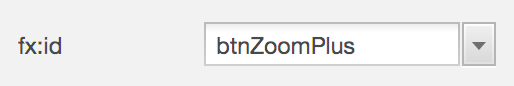
\includegraphics[]{images/fxid.png} 
	\captionof{figure}[]{Setzten der fx:id im SceneBuilder}
	\label{fig:fxid}
\end{figure}

Und hier das Beispiel im Code:
\begin{lstlisting}[caption= Beispielprogramm, label=lst:code]
	// Code ...
	
	@FXML
	private Button calculateButton; 
	
	// Code...
\end{lstlisting}

Weitere Informationen finden Sie in diesem Tutorial zu JavaFX.
\\
(http://code.makery.ch/library/javafx-8-tutorial/)

\paragraph{Apache Ant}
Apache Ant dient zur automatisierten Erstellung der ausführbaren Programme HPPLAN und CLSP aus einer gemeinsamen Code-Basis. Gleichzeitig werden Java-Docs erzeugt. 

Die ausführbare Software wird mit Hilfe von Build-Skripte erstellt, die alle Informationen zu benötigten Bibliotheken, Quelldateien und sonstigen einzubindenen Dateien beinhalten. Nachfolgende Abbildung gibt eine Übersicht über die für Ant notwendigen Dateien.

\begin{figure}[H]
	\centering
	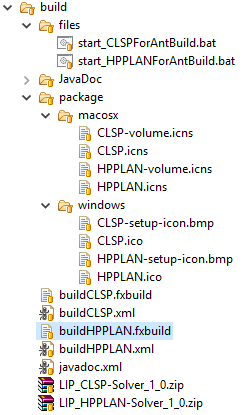
\includegraphics[]{images/antBuild.png} 
	\captionof{figure}[]{Dateien für Ant}
	\label{fig:antBuild}
\end{figure}

Der Ordner "'files"' enthält .bat Dateien für die Ausführung unter Windows. "'JavaDoc"' enthält die erzeugte Dokumentation zu Klassen und Methoden. In "'package"' sind Icon-Dateien für Windows und OSX hinterlegt. Mit Hilfe der Dateien "'buildCLSP.xml"' und "'buildHPPLAN.xml"' werden die Anwendungen erstellt. "'javadoc.xml"' erzeugt die Java-Dokumentation.

Nachfolgender Auszug aus der Build-Datei zu HPPLAN zeigt,wie die Main-Klasse festgelegt wird.

\begin{lstlisting}[caption= Ant Build-Skript HPPLAN, label=lst:code1]
	<!-- XML ... -->
	
	<fx:application id="fxApplication"
			name="${toolVersioned}"
			mainClass="de.oth.hsp.hpplan.HPPLANMain"
			version="${version}"
			toolkit="fx"
	/>
	
	<!-- XML... -->
\end{lstlisting}

Es ist wichtig, dass im jeweiligen Build-Skript die JDK Version von Java 8 übergeben wird. Folgendes Listing zeigt den XML-Code im Skript.

\begin{lstlisting}[caption= Ant Build-Skript mit Angabe der JDK Version, label=lst:code2]
	<!-- XML ... -->
	
	<javac includeantruntime="false" source="1.8" target="1.8" 
		   srcdir="build/src" destdir="build/classes" encoding="UTF-8">
		<classpath>
			<fileset dir="build/libs">
				<include name="*"/>
			</fileset>
		</classpath>
	</javac>
	
	<!-- XML ... -->
\end{lstlisting}

Ist dies gesetzt, können die Programme anschließend mit Hilfe der ausgegebenen BAT-Dateien gestartet werden.


\subsection{Komponenten}


\subsubsection{Allgemein}

Die unter der Komponente "'common"' zusammengefasste "'Komponenten"' enthalten die Hauptapplikation und geteilte Klassen für HPPLAN und CLSP.

\paragraph{common.dat}
Die Komponente "'dat"' enthält die Komponenten "'constraint"', "'parser"', "'parser.gen"' und "'value"'. Diese Komponenten sind notwendig für das Einlesen, Prüfen und Erstellen der DAT-Dateien, die dem ILOG-Framework übergeben werden.

\paragraph{common.ilog}
Festlegen von Schnittstellen für den Zugriff auf das Framework und die Entgegennahme von Ergebnissen von diesem. Weiterhin gibt es in der Komponente "'common.ilog.exception"' Klassen zur Fehlerbehandlung.

\paragraph{common.utils}
Diese Komponenten enthält Hilfsklassen für das Umwandeln von Arrays, dem Editieren einzelner Zellen in einer Tabelle und Dateioperationen.

\paragraph{common.view}
Enthält abstrakte Klassen und Methoden für Tabellen, die von den konkreten Klassen der View-Modelle von CLSP und HPPLAN geerbt werden, wenn diese eine Tabelle enthalten.

\subsubsection{HPPLAN}
Die Komponente "'hpplan"' enthält für das HPPLAN-Tool notwendigen Komponenten.

\paragraph{hpplan.ilog}
Diese Komponente umfasst alle Klassen, die für die Berechnung mit dem ILOG-Framework notwendig sind. "'HPPlanStatischModel"' beschreibt die MOD-Datei, die dem Framework übergeben wird. Weiterhin exisierten Klassen, die die Anfrage und das Rückgabeergebnis speichern. Die Klasse "'HPPlanStatischSolvingAlgorithm"' ist zuständig für die Kommunikation mit ILOG. Die Klassen dieser Komponente implementieren dabei die Schnittstellen aus der Komponente "'common.ilog"'. Zusätzlich sind zwei Hilfsklassen für die Bildung von Produkten enthalten.

\paragraph{hpplan.model}
Enthält die Klasse "'HpplanStatDatFile"', die eine Modell für das HPPLAN-Stat Problem enthält und vom ILOG-Framework zur Lösung des Problems benötigt wird.

\paragraph{hpplan.test}
Vorhanden, um die Anbindung an das Framework zu testen. Die enthaltene Klasse enthält Testdaten.

\paragraph{hpplan.view}
\label{par:hpplanView}
In dieser Komponente befinden sich die Controller und FXML Dateien der grafischen Oberfläche. Diese ist in ein RootLayout und zwei Reiter unterteilt. Das RootLayout definiert hier den Rahmen für die Reiter, die Menüleiste und die Unterleiste der Applikation.
\\
Die Reiter sind in das RootLayout integriert, besitzen aber eigene FXML-Dateien und Controller-Klassen. Dies wird im SceneBuilder wie folgt dargestellt:

\begin{figure}[H]
	\centering
	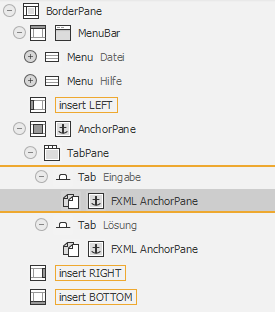
\includegraphics[]{images/fxTabs.png} 
	\captionof{figure}[]{Darstellung der Reiter im SceneBuilder}
	\label{fig:fxTabs}
\end{figure}

Damit die Unterkomponenten des RootLayout miteinander kommunizieren und aufeinander zugreifen können, wird ihnen der RootLayoutController übergeben. Dadurch ist es ihnen möglich auf die Elemente und Teile des RootLayout zuzugreifen.

Zur Eingabe der Daten enthält der Tab "'Eingabe"' 8 Unterseiten. Diese werden mit dem in Abbildung \ref{fig:hpplangui} am unteren Rand der Anwendung dargestellten PaginationController umgeschaltet. Dabei initialisiert und verwaltet die Klasse "'PaginationController"' die Unterseiten. Mit Hilfe eines Listeners wird der Wechsel einer Seite erkannt und durchgeführt.


\subsubsection{CLSP}
Die Komponente "'clsp"' enthält für das CLSP-Tool notwendigen Komponenten.

\paragraph{clsp.ilog}
Das CLSP-Model kann sowohl mit Gleitkommazahlen (Float) als auch Ganzzahlen (Integer) bestückt werden. Dafür gibt es zwei verschiedene Model-Klassen. Weiterhin exisitieren Klassen für die Anfrage und das Ergebnis des Algorithmus. Aufgrund der verschiedenen Modelle für CLSP gibt es auch zwei Klassen für die Kommunikation mit dem ILOG-Framework. Die genannten Klassen implementieren die dabei die allgemein definierten Schnittstellen aus "'common.ilog"', wobei die Schnittstelle "'ILogSolvingAlgorithm"' durch "'ICLSPSolvingAlgorithm"' erweitert werden. Es gibt außerdem eine Hilfsklasse für die Produktbildung.


\paragraph{clsp.model}
Enthält die Klasse "'ClspDatFile"', die eine Modell für das CLSP Problem enthält und vom ILOG-Framework zur Lösung des Problems benötigt wird.

\paragraph{clsp.test}
Vorhanden, um die Anbindung an das Framework zu testen. Die enthaltene Klasse enthält Testdaten.

\paragraph{clsp.view}
Siehe "'hpplan.view"' unter Abschnitt \ref{par:hpplanView}.


Nachfolgende Abbildungen gibt einen Überblick über die im Package-Explorer zu sehenden Komponenten. 

\begin{figure}[H]
	\centering
	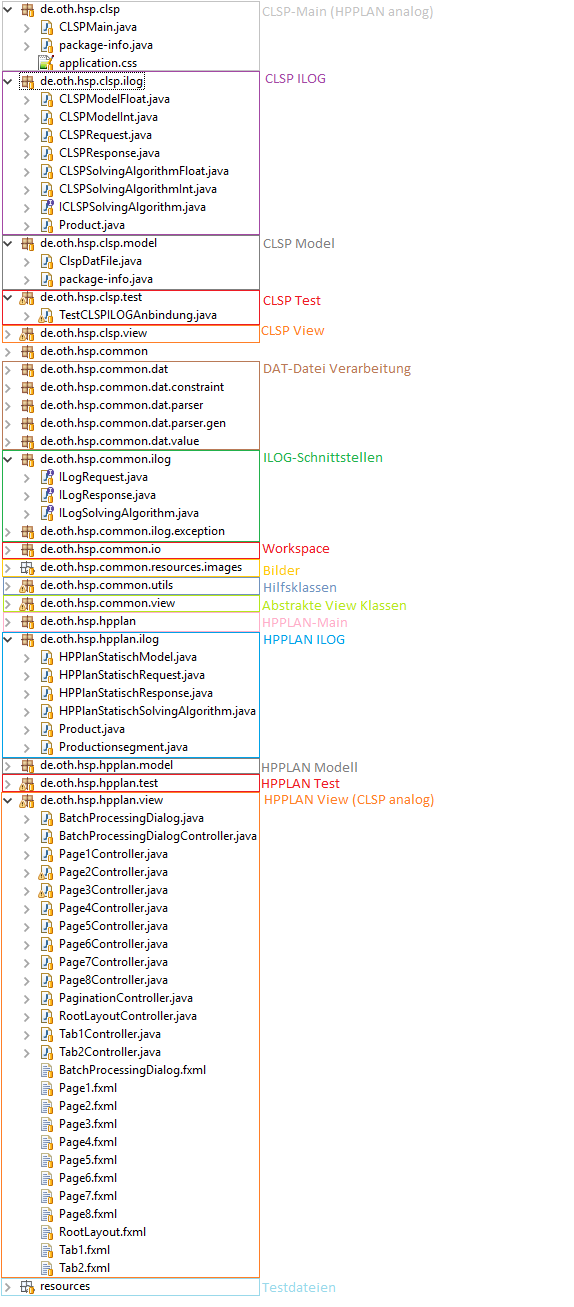
\includegraphics[scale=0.68]{images/komponenten.png} 
	\captionof{figure}[]{Komponenten im Package - Explorer}
	\label{fig:komponenten}
\end{figure}


%------------------------------------------------------------------------------
%	Implementierung
%------------------------------------------------------------------------------

\section{Implementierung}
Dieses Kapitel beschreibt die Implementierung, sowie die bei der Entwicklung der Komponenten verwendeten Bibliotheken. Die einzelnen Klassen werden in der Javadoc beschrieben.
 
\subsection{Verwendete Bibliotheken}
Die verwendeten Bibliotheken sind im Ordner lib gespeichert, um einen pfadunabhängigen Import in den Java Build Path zu ermöglichen. 
\\
Sie unterteilen sich in fünf Einsatzbereiche:
\begin{itemize}
	\item[JavaFX Zusätze:] Die hier verwendeten Bibliotheken erweitern JavaFX um vorgefertigte Dialoge und Buttons. Weitere Informationen unter: http://fxexperience.com/controlsfx/
	\item[ILOG-Framework:] Die ILOG-Framework Bilbiothek bildet die Schnittstelle zur ILOG Software.
	\item[ANTLR:] \gls{ANTLR} ist ein leistungsfähiger Parser zum lesen, verarbeiten, ausführen oder übersetzen von strukturiertem Text oder Binärdateien.
	\item[Apache Ant:] Die verwendeten Biliotheken werden für das Build-System Ant verwendet. Weitere Informationen unter: http://ant.apache.org/
	\item[Apache POI:] Ist eine freie Java Library, welche den Umgang mit Exceldateien ermöglicht. Benötigt wird dies dann, wenn das Framework keine ILog Installation auf dem Rechner findet. 
\end{itemize}

Nachfolgende Abbildung zeigt die verwendeten Bibliotheken in der Ordnerstruktur.
\begin{figure}[H]
	\centering
	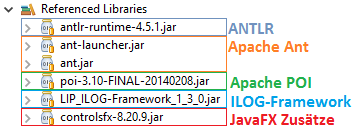
\includegraphics[width=0.9\linewidth]{images/libs.png} 
	\captionof{figure}[]{Verwendete Bibliotheken}
	\label{fig:libs}
\end{figure}

In den folgenden Abschnitten werden einige ausgewählte Programmabläufe detaillierter beschrieben. Dabei steht vor allem der Umgang mit den DAT-Dateien und das Anstoßen der Berechnung im Vordergrund. Die Erzeugung von DAT-Dateien und das Laden dieser wird anhand von CLSP erklärt und ist zum Vorgehen in HPPLAN analog. 

\subsection{Erzeugung DAT-Dateien}
Es besteht die Möglichkeit eingegebene Werte in einer DAT-Datei zu speichern und diese bei Bedarf wieder einzulesen (siehe \ref{subsec:ladenDat}). Das Speichern von Dateien wird dabei in der Klasse "'RootLayoutController"' durchgeführt. Nachfolgend wird das Vorgehen der Erzeugung grob beschrieben.

\begin{enumerate}
	\item Im Untermenü Datei wird die Funktion Speichern angewählt, wodurch im\\ "'RootLayoutController"' die Methode "'onActionFileSave"' aufgerufen wird.
	\item Es wird ein Dialog zum Speichern angezeigt, der dem Benutzer die Wahl über den Speicherort und den Dateinamen gibt.
	\item Eine leere Datei vom Typ "'.dat"' wird angelegt.
	\item Alle im aktuellen CLSP-Modell enthaltenen Werte werden in der DAT-Datei gespeichert.
\end{enumerate}

Die gespeicherten Dateien haben dabei nachfolgenden Inhalt und sind je nach eingegebenen Dateien befüllt.

\begin{lstlisting}[caption= Inhalt DAT-Datei, label=lst:dat]
CPLEX_EPGAP =0.0001;
// Anzahl Perioden:
T=2;
// Anzahl Produkte:
K=2;
//Ressource
J=2;
//grosse zahl
M=5768668;

//kapazitaeten
b= #[ 
1: [3000 3000]
2: [3000 3000]
]#;


// Bedarfe je Produkt und Periode:
d= #[ 
1: [20 30]
2: [20 50]
]#;
// Lagerkosten:
h= [2 2]; 
// Ruestkosten:
s= [200 200]; 
// Stueckbearbeitungszeit je Produkt und Ressource:
tb= #[ 
1: [20 30]
2: [20 50]
]#;
// Ruestzeit je Produkt und Ressource:
tr= #[ 
1: [20 30]
2: [20 50]
]#;
//mindestvorlaufzeiten
z= [0 0];
// Anfangslagerbestaende:
y0 = [10 0];
// Endlagerbestaende:
yT = [30 0];
\end{lstlisting}


\subsection{Laden von DAT-Dateien}
\label{subsec:ladenDat}

Das Laden von Dateien wird ebenfalls mit durch die Klasse "'"' angetriggert. Im Zuge dessen wird die allgemeine Komponente "'common.data"' und ihre Unterkomponenten zum Parsen der Dateien verwendet. Nachfolgend wird der Ablauf beschrieben.

\begin{enumerate}
	\item Im Untermenü Datei wird die Funktion Öffnen angewählt, wodurch im\\ "'RootLayoutController"' die Methode "'onActionFileOpen"' aufgerufen wird.
	\item Es wird ein Öffnen-Dialog gestartet mit dem die zu öffnende Datei ausgewählt wird.
	\item Mit Hilfe der in beiden Tools verwendeten Klasse "'DatFileParser"' wird die gewählte Datei eingelesen und ein Modell vom Typ "'ClspDatFile"' oder "'HpplanStatDatFile"' zurückgegeben. 
	\item Die aktuelle Seite wird mit den neuen Werten befüllt. (Beim Aufruf einer Seite werden die Werte stets aus dem Modell geladen)
\end{enumerate}


\subsection{Berechnung}
Nachfolgend werden sowohl für CLSP als auch HPPLAN grob die Berechnungschritte aufgezeigt. Die Berechnung wird in beiden Tools auf Seite 8 des Tabs Eingabe durch den Button "'Berechnung starten"' ausgelöst. Dabei wird die Aktion an die Methode "'calculateCLSP"' oder "'calculateHPPLAN"' des "'RootLayController"'durchgereicht.

\subsubsection{CLSP}
Anders als bei HPPLAN kann im CLSP Tool eine weitere Einstellung vorgenommen werden. Unter Optionen\textbackslash Algorithmuseinstellung kann zwischen Ganzzahl und Kommazahl in der Berechnung gewählt werden.

Nachfolgend werden die Schritte der Berechnung in der CLSP Anwendung aufgezeigt.

\begin{enumerate}
	\item Das Modell wird erneut gespeichert, damit alle Werte aktuell sind.
	\item Je nach Algorithmuseinstellung wird eine Instanz der Klasse "'CLSPSolvingAlgorithmInt"' für die Ganzzahlberechnung oder "'CLSPSolvingAlgorithmFloat"' für die Gleitkommaberechnung angelegt.
	\item Das Modell wird in ein Request-Objekt "'CLSPRequest"' geschrieben und der Algorithmus-Klasse zur Lösung übergeben.
	\item Das Problem wird mit Hilfe von ILOG gelöst.
	\item Die Lösung von ILOG wird in das Objekt "'CLSPResponse"' geschrieben.
	\item Das Ergebnis wird unter dem Tab "'Lösung"' dargestellt.
\end{enumerate}

\subsubsection{HPPLAN}
Nachfolgend werden die Schritte der Berechnung in der CLSP Anwendung aufgezeigt.

\begin{enumerate}
	\item Das Modell wird erneut gespeichert, damit alle Werte aktuell sind.
	\item Es wird ein Instanz der Klasse "'HPPlanStatischSolvingAlgorithm"' erzeugt.
	\item Das Modell wird in ein Request-Objekt "'HPPlanStatischRequest"' geschrieben und der Algorithmus-Klasse zur Lösung übergeben.
	\item Das Problem wird mit Hilfe von ILOG gelöst.
	\item Die Lösung von ILOG wird in das Objekt "'HPPlanStatischResponse"' geschrieben.
	\item Das Ergebnis wird unter dem Tab "'Lösung"' dargestellt.
\end{enumerate}

%TODO Bild Lösung in Software CLSP oder HPPLAN

\subsection{Stapelverarbeitung}
%TODO Geht noch nicht, Prinzip beschreiben
Der Menüpunkt Datei\textbackslash Stapelverarbeitung ist in beiden Anwendungen vorhanden. Beim Auswählen des Menüpunktes wird ein Dialog geöffnet in dem mehrere Dateien zur Verarbeitung und ein Ziel zum Abspeichern der Ergebnisse ausgewählt werden können.
\\
Es werden dabei bereits Ordner erzeugt und die Berechnung der Ergebnisse aus den gewählten DAT-Dateien ist implementiert. Jedoch ist es mit dem zum Zeitpunkt der Entwicklung zur Verfügung stehenden ILOG-Framework nicht möglich, die Ergebnisse in Excel-Dateien zu speichern. Dadurch ist es nicht möglich eine Stapelverarbeitung sinnvoll durchzuführen.


%-------------------------------------------------------------------------------------
% Verzeichnisse %-------------------------------------------------------------------------------------
%	\rhead{Verzeichnisse} %Kopftextbeschriftung
%
%	\stepcounter{section}
%	\phantomsection \label{Verzeichnisse}
%	\addcontentsline{toc}{section}{Verzeichnisse} %Ohne Nummer ins Inhaltsverzeichnis
%	\renewcommand{\thesection}{\Roman{verzeichnis}}
	
	% Abkürzungen
%	\stepcounter{verzeichnis}
	\newpage
	\section{Abkürzungsverzeichnis}
	\vspace{-6em} % Abstand analog der anderen Verzeichnisse reduzieren
	\printnoidxglossary[type=\acronymtype,style=alttree,title=,toctitle=] %automatischen Titel und Gliederungsbeschriftung unterdrücken - sonst steht da Glossarie
	


\end{document}
